%!TEX root = htm.tex
\section{Progressive HyTM must perform incremental validation}
\label{sec:lb}
%
%
In this section, we show that it is impossible to implement opaque \emph{progressive} HyTMs with \emph{invisible reads}
with $O$(1) step-complexity read operations for slow-path transactions. 
This result holds even if fast-path transactions may perform
direct trivial accesses.

Formally, we say that a HyTM implementation $\mathcal{M}$ is progressive
for a set $\mathcal{T}$ of transactions
if in any execution $E$ of $\mathcal{M}$; $\mathcal{T} \subseteq \ms{txns}(E)$, 
if any transaction $T_k \in \mathcal{T}$ returns $A_k$ in $E$, there exists 
another concurrent transaction $T_m$ that \emph{conflicts} (both access the same t-object and at least one writes) with $T_k$ in $E$~\cite{tm-book}.

We construct an execution of a progressive opaque HyTM in which every t-read performed by a read-only slow-path transaction
must access linear (in the size of the read set) number of distinct base objects.
%
\begin{theorem}
\label{th:impossibility}
Let $\mathcal{M}$ be any progressive opaque HyTM implementation providing invisible reads.
There exists an execution $E$ of $\mathcal{M}$ and some slow-path read-only transaction $T_k \in \ms{txns}(E)$
that incurs a time complexity of $\Omega (m^2)$; $m=|\Rset(T_k)|$.
\end{theorem}
%
\begin{proofsketch}
We construct an execution of a read-only slow-path transaction $T_{\phi}$ that performs $m \in \mathbb{N}$
distinct t-reads of t-objects $X_1,\ldots , X_m$. We show inductively that for each 
$i\in \{1,\ldots , m\}$; $m \in \mathbb{N}$, the $i^{\ms{th}}$ t-read must access $i-1$ distinct base objects
during its execution. The (partial) steps in our execution are depicted in Figure~\ref{fig:indis}.

For each $i\in \{1,\ldots , m\}$, $\mathcal{M}$ has an execution of the form depicted in Figure~\ref{sfig:inv-2}.
Start with the complete step contention-free execution of slow-path read-only transaction $T_{\phi}$ that performs
$(i-1)$ t-reads: $\Read_{\phi}(X_1)\cdots \Read_{\phi}(X_{i-1})$, followed by the t-complete step contention-free execution of a fast-path transaction $T_{i}$
that writes $nv_i\neq v_i$ to $X_i$ and commits and then the complete step contention-free execution fragment of $T_{\phi}$ that performs its $i^{th}$ t-read:
$\Read_{\phi}(X_i) \rightarrow nv_i$. Indeed, by progressiveness, $T_i$ cannot incur tracking set aborts and since it accesses only a single t-object, it cannot incur capacity aborts.
Moreover, in this execution, the t-read of $X_i$ by slow-path transaction $T_{\phi}$ must return the value $nv$ written by fast-path transaction $T_i$ since this execution is indistinguishable
to $T_{\phi}$ from the execution in Figure~\ref{sfig:inv-1}. 
Finally, we construct $(i-1)$ different executions of the form depicted in Figure~\ref{sfig:inv-3}: for each $\ell \leq (i-1)$, 
a fast-path transaction $T_{\ell}$ (preceding $T_i$ in real-time ordering, but invoked following the $(i-1)$ t-reads by $T_{\phi}$) writes $nv_{\ell}\neq v$ to $X_{\ell}$ and commmits, followed by
the t-read of $X_i$ by $T_{\phi}$. Observe that, $T_{\ell}$ and $T_i$ which access mutually disjoint data sets cannot contend on each other since if they did, they would concurrently contend
on some base object and incur a tracking set abort, thus violating progressiveness.
Indeed, by the TM-liveness property we assumed (cf. Section~\ref{sec:hytm} and invisible reads for $T_{\phi}$, each of these $(i-1)$ executions exist. 

In each of these $(i-1)$ executions, t-read of $X_i$ cannot return the new value $nv$:
the only possible serialization for transactions is $T_{\ell}$, $T_i$, $T_{\phi}$; but $\Read_{\phi}(X_{\ell})$
performed by $T_k$ that returns the initial value $v$ is not legal in this serialization---contradiction to the assumption of opacity.
In other words, slow-path transaction $T_{\phi}$ is forced to verify the validity of t-objects in $\Rset(T_{\phi})$.
Finally, we note that, for all $\ell, \ell' \leq (i-1)$;$\ell' \neq \ell$, 
fast-path transactions $T_{\ell}$ and $T_{\ell'}$ access mutually disjoint sets of base objects thus forcing the t-read of $X_i$ to access least $i-1$ different base objects
in the worst case.
Consequently, for all $i \in \{2,\ldots, m\}$, slow-path transaction $T_{\phi}$ must perform at least $i-1$ steps 
while executing the $i^{th}$ t-read in such an execution.
\end{proofsketch}
%
%
\vspace{1mm}\noindent\textbf{How STM implementations mitigate the lower bound cost.}
NOrec~\cite{norec} is a progressive opaque STM that minimizes the average step-complexity resulting from incremental 
validation of t-reads. Transactions read a global versioned lock at the start, and perform value-based validation
during t-read operations \emph{iff} the global version has changed.
TL2~\cite{DSS06} improves over NOrec by circumventing the lower bound
of Theorem~\ref{th:impossibility}. Concretely, TL2 associates a global version with each t-object updated during
a transaction and performs validation with O(1) complexity during t-reads by simply verifying if the version
of the t-object is greater than the global version read at the start of the transaction. Technically,
NOrec and algorithms in this paper provide a stronger definition of progressiveness: a transaction may abort
only if there is a prefix in which it conflicts with another transaction and both are t-incomplete. TL2 on the other hand allows
a transaction to abort due to a concurrent conflicting transaction.

\vspace{1mm}\noindent\textbf{Implications for disjoint-access parallelism in HyTM.}
The property of disjoint-access parallelism (DAP), in its \emph{weakest} form, ensures that two transactions %$T_1$ and $T_2$
concurrently contend on the same base object 
%(both access the base object and at least one updates it) 
only if their data 
sets are connected in the \emph{conflict graph}, capturing 
data-set overlaps among all concurrent transactions~\cite{AHM09}. It is well known that weak DAP STMs with invisible reads must perform incremental validation even if the required TM-progress condition requires
transactions to commit only in the absence of any concurrent transaction~\cite{tm-book,prog15-pact}. For example, DSTM~\cite{HLM+03} is a weak DAP STM that is progressive and consequently incurs the validation
complexity. On the other hand, TL2 and NOrec are not weak DAP since they employ a global versioned lock that mitigates the cost of incremental validation, but this allows two transactions accessing
disjoint data sets to concurrently contend on the same memory location. Indeed, this inspires the proof of Theorem~\ref{th:impossibility}. 
%%%%%%%%%%%%%%%%%%%%%%%%%%%%%%%%%%%%%
\begin{figure*}[!t]
\begin{center}
	\subfloat[Slow-path transaction $T_{\phi}$ performs $i-1$ distinct t-reads (each returning the initial value) followed by the t-read of $X_i$ that returns value $nv$ 
	writtten by fast-path transaction $T_i$\label{sfig:inv-1}]{\scalebox{0.6}[0.6]{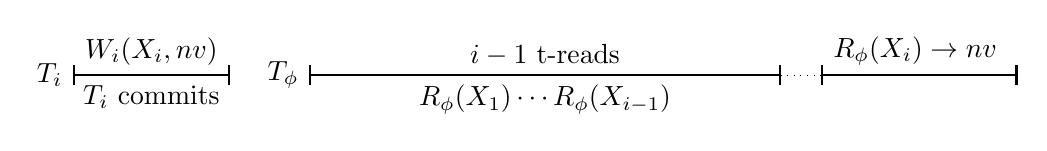
\begin{tikzpicture}
\node (r1) at (3,0) [] {};
\node (r2) at (7.7,0) [] {};

\node (w1) at (-2,0) [] {};


\draw (r1) node [below] {\normalsize {$R_{\phi}(X_1) \cdots R_{\phi}(X_{i-1})$}};
\draw (r1) node [above] {\normalsize {$i-1$ t-reads}};

\draw (r2) node [above] {\normalsize {$R_{\phi}(X_i)\rightarrow nv$}};

\draw (w1) node [above] {\normalsize {$W_i(X_i,nv)$}}; 
\draw (w1) node [below] {\normalsize {$T_i$ commits}};


\begin{scope}   
\draw [|-|,thick] (0,0) node[left] {$T_{\phi}$} to (6,0);
\draw [|-|,thick] (6.5,0) node[left] {} to (9,0);
\draw [-,dotted] (0,0) node[left] {} to (9,0);
\end{scope}
%
%
\begin{scope}   
%\draw [|-|,thick] (0,0) node[left] {$T_k$} to (6,0);
\draw [|-|,thick] (-3,0) node[left] {$T_i$} to (-1,0);
\end{scope}
%
\end{tikzpicture}
}}
        \\
        \vspace{1mm}
	\subfloat[Fast-path transaction $T_i$ does not contend with any of the $i-1$ t-reads performed by $T_{\phi}$;
	this execution is indistinguishable to $T_{\phi}$ from \ref{sfig:inv-1} and t-read of $X_i$ must return $nv$\label{sfig:inv-2}]{\scalebox{0.6}[0.6]{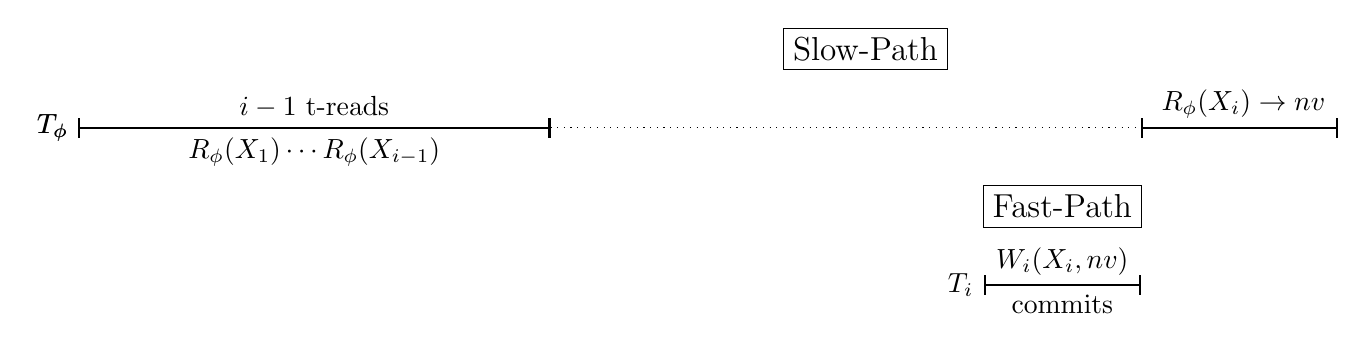
\begin{tikzpicture}
\node (r1) at (3,0) [] {};
%\node (r2) at (7.7,0) [] {};
\node (r3) at (14.8,0) [] {};

%\node (w1) at (7.5,-2) [] {};

\node (w2) at (12.5,-2) [] {};

\draw (r1) node [below] {\normalsize {$R_{\phi}(X_1) \cdots R_{\phi}(X_{i-1})$}};
\draw (r1) node [above] {\normalsize {$i-1$ t-reads}};

\draw (w2) node [above] {\normalsize {$W_{i}(X_{i},nv)$}}; 
\draw (w2) node [below] {\normalsize {commits}};

\draw (r3) node [above] {\normalsize {$R_{\phi}(X_{i})\rightarrow nv$}};
\node[draw,align=left] at (10,1) {{\large Slow-Path}};
\node[draw,align=left] at (12.5,-1) {{\large Fast-Path}};


\begin{scope}   
\draw [|-|,thick] (0,0) node[left] {$T_{\phi}$} to (6,0);
\draw [|-|,dotted] (0,0) node[left] {$T_{\phi}$} to (16,0);
\draw [|-|,thick] (13.5,0) node[left] {} to (16,0);
\end{scope}
%
%
\begin{scope}   
%\draw [|-|,thick] (0,0) node[left] {$T_k$} to (6,0);
\draw [|-|,thick] (11.5,-2) node[left] {$T_i$} to (13.5,-2);
\end{scope}
%
\end{tikzpicture}
%}}
	\\
	\vspace{1mm}
	\subfloat[To distinguish the $i-1$ different executions, t-read of $X_i$ by slow-path transaction $T_{\phi}$ is forced
	to access $i-1$ different base objects\label{sfig:inv-3}]{\scalebox{0.6}[0.6]{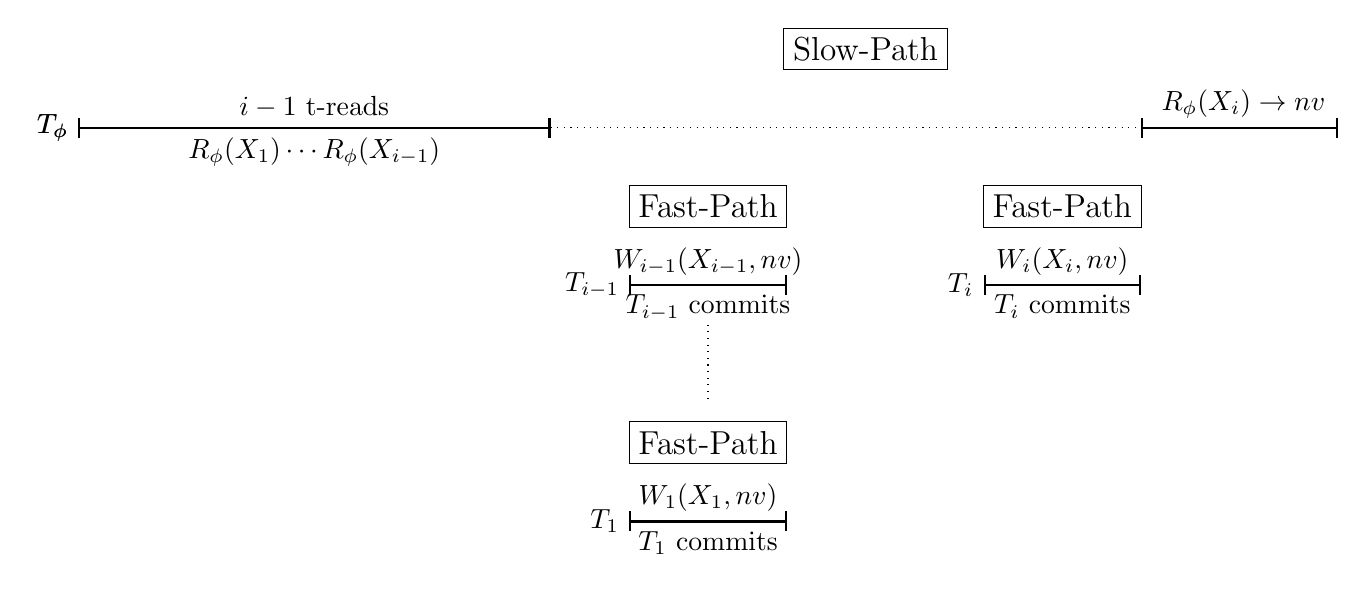
\begin{tikzpicture}
\node (r1) at (3,0) [] {};
%\node (r2) at (7.7,0) [] {};
\node (r3) at (14.8,0) [] {};


\node (w2) at (12.5,-2) [] {};
\node (w3) at (8,-2) [] {};
\node (w4) at (8,-5) [] {};


\draw (r1) node [below] {\normalsize {$R_{\phi}(X_1) \cdots R_{\phi}(X_{i-1})$}};
\draw (r1) node [above] {\normalsize {$i-1$ t-reads}};

\draw (w2) node [above] {\normalsize {$W_{i}(X_{i},nv)$}}; 
\draw (w2) node [below] {\normalsize {$T_{i}$ commits}};

\draw (w3) node [above] {\normalsize {$W_{i-1}(X_{i-1},nv)$}}; 
\draw (w3) node [below] {\normalsize {$T_{i-1}$ commits}};

\draw (w4) node [above] {\normalsize {$W_{1}(X_{1},nv)$}}; 
\draw (w4) node [below] {\normalsize {$T_{1}$ commits}};

\draw (r3) node [above] {\normalsize {$R_{\phi}(X_{i})\rightarrow nv$}};
\node[draw,align=left] at (10,1) {{\large Slow-Path}};
\node[draw,align=left] at (12.5,-1) {{\large Fast-Path}};
\node[draw,align=left] at (8,-1) {{\large Fast-Path}};
\node[draw,align=left] at (8,-4) {{\large Fast-Path}};
\begin{scope}   
\draw [|-|,thick] (0,0) node[left] {$T_{\phi}$} to (6,0);
\draw [|-|,dotted] (0,0) node[left] {$T_{\phi}$} to (16,0);
\draw [|-|,thick] (13.5,0) node[left] {} to (16,0);
\end{scope}
%
%
\begin{scope}   
\draw [|-|,thick] (7,-2) node[left] {$T_{i-1}$} to (9,-2);
\draw [|-|,thick] (11.5,-2) node[left] {$T_i$} to (13.5,-2);
\draw [-,dotted] (8,-2.5)  to (8,-3.5);
\draw [|-|,thick] (7,-5) node[left] {$T_1$} to (9,-5);

\end{scope}
%
\end{tikzpicture}
%}}
	\caption{Proof steps for Theorem~\ref{th:impossibility}
        \label{fig:indis}} 
\end{center}
\end{figure*}
